% IEEE standard conference template; to be used with:
%   spconf.sty  - LaTeX style file, and
%   IEEEbib.bst - IEEE bibliography style file.
% --------------------------------------------------------------------------

\documentclass[letterpaper]{article}
\usepackage{spconf,amsmath,amssymb,graphicx}
\usepackage[utf8]{inputenc}
\usepackage[linesnumbered, ruled]{algorithm2e}

% Example definitions.
% --------------------
% nice symbols for real and complex numbers
\newcommand{\R}[0]{\mathbb{R}}
\newcommand{\C}[0]{\mathbb{C}}

% bold paragraph titles
\newcommand{\mypar}[1]{{\bf #1.}}

% Title.
% ------
\title{A parallel implementation of the Gumtree Algorithm in C++}
%
% Single address.
% ---------------
%\name{Balz Guenat, Christopher Signer, Amirreza Bahreini}
\name{Balz Guenat, Christopher Signer}
\address{Department of Computer Science\\ ETH Zürich\\Zürich, Switzerland}

% For example:
% ------------
%\address{School\\
%		 Department\\
%		 Address}
%
% Two addresses (uncomment and modify for two-address case).
% ----------------------------------------------------------
%\twoauthors
%  {A. Author-one, B. Author-two\sthanks{Thanks to XYZ agency for funding.}}
%		 {School A-B\\
%		 Department A-B\\
%		 Address A-B}
%  {C. Author-three, D. Author-four\sthanks{The fourth author performed the work
%		 while at ...}}
%		 {School C-D\\
%		 Department C-D\\
%		 Address C-D}
%

\begin{document}
%\ninept
%
\maketitle
%

\begin{abstract}
%The evolution of software projects is recorded with version control systems which store snapshots of the project at different points in time. To help developers understand the transitions between these snapshots, \emph{diff} programs are used to highlight the differences between them. In an effort to provide developers with a better description of these differences the \emph{Gumtree} algorithm computes a matching between the nodes of the abstract syntax trees of the two snapshots.

\emph{Gumtree} is an algorithm to compute a matching between the nodes of two similar abstract syntax trees.
It was developed with the goal of improving code differencing tools used with version control systems and the original authors have written a single-threaded implementation in Java.
Their evaluation showed that the \emph{Gumtree} algorithm is significantly slower than traditional \emph{diff} tools.
To alleviate this disadvantage we implement the algorithm in C++, parallelize the computation where possible and introduce an algorithmic optimization that effectively reduces the algorithmic complexity of a subprocedure  from $O(n^2)$ to $O(n)$.
Our evaluation shows that on randomly generated problem instances and real world examples our implementation runs multiple times faster than the Java implementation but benefits little from multithreading.
We argue that the greedy nature of the algorithm prevents an effective utilization of multiple threads.
\end{abstract}

\section{Introduction}\label{sec:intro}

%In this section we explain the problem the \emph{Gumtree} algorithm attempts to solve and state the goal of our work.

Software projects evolve over the time of their development and operation.
Nowadays the history of such evolution is typically recorded by a version control system (VCS) which stores snapshots of the project state.
For the developers to understand this evolution, it is of tremendous help if not only these snapshots are available but also a representation of the transitions between them.
Often these transitions are represented in form of differences between the files or as edit operations transforming the old state into the new state.

The transitions are usually not stored explicitly but are computed from the two states at the user's request.
Algorithms performing this computation are called \emph{diff algorithms}.
Most popular diff algorithms like \emph{GNU diff}, \emph{KDiff3} and \emph{git-diff} regard files as lists of lines and find the differences between them by computing their longest common subsequence and regarding those lines as unchanged.

This approach is simple and fast but it is often too coarse grained and lacks conciseness.
Consider for example the definition of a Java method that is moved from the top of a file to the bottom of the same file.
\emph{git-diff} will regard this as a deletion of multiple lines at the top of the file and an unrelated addition of multiple lines at the bottom.

Falleri et al. \cite{falleri:2014:structure_diff} propose an approach to code differencing that leverages the structure inherent in program code in an attempt to overcome these issues.
Instead of regarding files as lists of lines, the code is parsed to yield an abstract syntax tree (AST).
Then, to find the unchanged parts of the code, a matching between the two versions of the AST is computed and finally a description of edit operations is generated.
The main contribution of the paper is the \emph{Gumtree} algorithm which is used to find said matching.
Using this structure-aware approach, the example from before will result in a single move operation of the AST node representing the method definition.

The disadvantages of this approach are twofold.
Firstly, it requires the integration of a parser for the respective language to generate the AST.
Secondly, parsing and subsequently finding a matching between the ASTs is more computationally involved and thus takes a longer time than traditional approaches.
The paper reports an increase of execution time by factors 18 and 30, for a Java and JavaScript project respectively, compared to a textual diff program.
Parsing accounts for around 55\% and 33\% of the total execution time.
When testing the performance of the given Java implementation on a C++ project, we found that the execution time increases drastically to the point where practical application is impossible.
%The existing Java implementation\footnote{github.com/GumTreeDiff/gumtree} defers the generation of the AST to an external component so its overall performance is partially out of its control.
%The matching itself is computed in a purely single-threaded manner.
In an attempt to alleviate this performance disadvantage, we implement the \emph{Gumtree} algorithm in C++, optimize it and attempt to further increase the performance by parallelizing it where possible.
We use the existing Java implementation as a reference both in terms of correctness as well as performance.

\section{Background: The Gumtree algorithm}\label{sec:background}

This section describes the original \emph{Gumtree} algorithm as it was introduced in sections 2 and 3 in the Falleri paper \cite{falleri:2014:structure_diff}. The authors provide an openly available Java implementation on Github\footnote{github.com/GumTreeDiff/gumtree}.

\mypar{Problem definition}
The \emph{Gumtree} algorithm regards ASTs as ordered rooted trees where nodes have a type and may have a string token associated to them.
%It was designed specifically with ASTs in mind but can be applied to any type of tree with these properties.
Given two such trees $T_1$ and $T_2$, the algorithm produces a matching between the nodes of the two trees.
A matching is represented as a set of pairs of nodes where each node is part of at most one pair and nodes belonging to the same pair have the same type.

\mypar{Algorithm overview}
The algorithm computes such a matching in two successive phases:
\begin{enumerate}
	\item The top-down phase in which isomorphic subtrees are found and matched.
	\item The bottom-up phase in which nodes are matched if many of their descendants have already been matched.
\end{enumerate}
The Falleri paper additionally describes the search for so-called \emph{recovery mappings} in the second phase.
We omit this step as it requires the implementation of a separate optimal algorithm which we deemed out of scope for this project.
For the purpose of comparing our implementation to the reference, we have modified the original implementation to omit this step as well.

\mypar{Top-down phase}
This phase finds and matches isomorphic subtrees down to a minimum height $minHeight$ by comparing increasingly smaller subtrees.
Unique matches are accepted immediately while subtrees that are isomorphic to multiple subtrees are matched based on the similarity of their parents at a later stage.
Two subtrees with roots $t_1$ and $t_2$ are isomorphic if and only if $t_1$ and $t_2$ have the same type and token and every child of $t_1$ is isomorphic to the respective child of $t_2$.

This phase uses a height-indexed priority list of subtrees (each represented by its root node) for each input tree supporting the following operations:
\emph{peekMax} returns the maximum subtree height in the list.
\emph{pop} returns the set of subtrees with maximum height and removes them from the list.
\emph{push} inserts a subtree into the list.
\emph{open} inserts all children of a node into the list.

Further we define a similarity function $sim$ on subtrees given a mapping $M$ as follows:
$$ sim(t_1, t_2, M) = \frac{| \{ t_x \in d(t_1), t_y \in d(t_2) : (t_x, t_y) \in M \} | }{ (|d(t_1)| + |d(t_2)|) / 2} $$
where $d(t)$ is the set of descendants of $t$. $sim$ rates the similarity of two subtrees in the range $[0,1]$ where a value of 1 indicates that the two nodes have the same descendants.
When a given node can be matched to multiple nodes we use this similarity measure on the parents of the candidates to decide between them.

See Algorithm \ref{alg:top-down} for a full description of the top-down phase.

\SetKw{KwOr}{or}
\SetAlFnt{\footnotesize}
\SetInd{0.3em}{0.6em}
\SetAlgoVlined

\begin{algorithm}
	\KwData{Two trees $T_1, T_2$, a minimum height $minHeight$, two empty height-indexed priority lists $L_1, L_2$, an empty list of candidate mappings $A$ and an empty set of mappings $M$}
	\KwResult{The set of mappings $M$}
	push(root($T_1$), $L_1$)\;
	push(root($T_2$), $L_2$)\;
	\While{$ min(peekMax(L_1),peekMax(L_2)) > minHeight $}{
		\eIf{$ peekMax(L_1) \neq peekMax(L_2) $}{
			\eIf{$ peekMax(L_1) > peekMax(L_2) $}{
				\lForEach{$ t \in pop(L_1) $}{
					$open(t,L_1)$
					}
				}{
				\lForEach{$ t \in pop(L_2) $}{
					$open(t,L_2)$
					}
				}
		}{
			$H_1 \gets pop(L_1)$\;
			$H_2 \gets pop(L_2)$\;
			\ForEach{$ (t_1,t_2) \in H_1 \times H_2 $}{
				\If{$ \text{isomorphic}(t_1,t_2) $}{
					\eIf{$ \exists t_y \in H_2 : \text{isomorphic}(t_1,t_y) \wedge t_y \neq t_2 $\\ \KwOr $ \exists t_x \in H_1 : \text{isomorphic}(t_x,t_2) \wedge t_x \neq t_1 $\\}{
						add($A, (t_1,t_2)$)\;
					}{
						add all pairs of isomorphic nodes of $d(t_1)$ and $d(t_2)$ to $M$\;
					}
				}{
				}
			}
			\lForEach{$ t_1 \in H_1 : (t_1,t_y) \notin A \cup M $}{$ \text{open}(t_1,L_1) $}
			\lForEach{$ t_2 \in H_2 : (t_x,t_2) \notin A \cup M $}{$ \text{open}(t_2,L_2) $}
		}
	}
	sort $(t_1,t_2) \in A$ using $sim(parent(t_1),parent(t_2), M)$\;
	\While{$\text{size}(A) > 0$}{
		$(t_1,t_2) \gets \text{popLargest}(A)$\;
		add all pairs of isomorphic nodes of $d(t_1)$ and $d(t_2)$ to $M$\;
		$A \gets A \setminus \{(t_1,t_y) \in A\}$\;
		$A \gets A \setminus \{(t_x,t_2) \in A\}$\;
	}
\caption{The top-down phase}
\label{alg:top-down}
\end{algorithm}

\mypar{Bottom-up phase}
The bottom-up phase takes the mappings computed by the top-down phase as input.
$T_1$ is traversed in post-order and for each non-leaf node $t_1$ that has not been matched yet, a list of candidate nodes from $T_2$ is computed.
A node $c \in T_2$ is a candidate for $t_1$ if it is unmatched, has the same type as $t_1$ and has some matching descendants.
$t_1$ is then matched with the candidate with the largest similarity value $sim(t_1,c,M)$ provided it is over a certain threshold $minSim$.

See Algorithm \ref{alg:bottom-up} for a full description of the bottom-up phase.
The mapping $M$ resulting from this phase is the final output of the \emph{Gumtree} algorithm without \emph{recovery mappings}.

\begin{algorithm}
	\KwData{Two trees $T_1, T_2$, a set of mappings $M$ (from the top-down phase), two lists of nodes $seeds, candidates$ and a threshold $minSim$}
	\KwResult{The set of mappings $M$}
	\ForEach{$t_1 \in T_1$ in post-order}{
		\If{$t_1$ is not matched $\wedge t_1$ has matched children}{
			%$t_2 \gets \text{bestCandidate}(t_1,M)$\;
			$seeds \gets \{t_2 : (c_1, t_2) \in M \wedge c_1 \in d(t_1) \}$\;
			\ForEach{$s \in seeds$}{
				\While{$s \neq root(T_2)$}{
					$s \gets parent(s)$\;
					\If{$ type(s) = type(t_1) \wedge s \neq root(T_2) \wedge $ $s \text{ is not matched} $}{
						add($candidates, s$)\;
					}
				}
			}
			\If{$candidates \neq \emptyset $}{
				%$t_2 \gets \{c \in candidates : c \text{ maximises } sim(t_1, c, M)\}$\;
				$t_2 \gets c \in candidates$ with maximum $sim(t_1,c,M)$\;
				\If{$ sim(t_1,t_2,M) > minSim $}{
					add $(t_1,t_2)$ to $M$\;
				}
			}
		}
	}
\caption{The bottom-up phase (without \emph{recovery mappings})}
%\caption{The bottom-up phase}
\label{alg:bottom-up}
\end{algorithm}

\mypar{Chosen thresholds}
We set the named thresholds to $minSim=0.5$ and $minheight=2$ as recommended in the Falleri paper \cite{falleri:2014:structure_diff}.

\section{Implementation}\label{sec:yourmethod}

In this section we present our implementation of the \emph{Gumtree} algorithm written in C++ and describe our efforts to optimize and parallelize it.
To achieve parallelization, we make use of the OpenMP API\footnote{openmp.org}.
The entire project is open source and available on Github\footnote{github.com/BalzGuenat/ParallelGumtree}.

\mypar{Writing Gumtree in C++}
To write our implementation we adhered very closely to the existing Java implementation of the matching algorithm.
Besides the matching algorithm the Java implementation also features a framework for easier integration of parsers and other components.
In our work we focus only on the matching algorithm.
To avoid the integration of a parser we use a simple encoding format for the input trees that stores each node on a line.
We output the resulting matching as tuples of line numbers identifying the nodes in the input trees.

For the purpose of testing and evaluating our implementation we implement two components for the Java implementation.
The first component parses the mentioned encoding format and constructs the tree objects used by the matching algorithm.
The second components simply writes the resulting matching to a file, again in the same format as the C++ implementation.
The code for these component is available on Github\footnote{github.com/BalzGuenat/gumtree/tree/prallel-gt-reference}.

\mypar{Search space reduction}
In the top-down phase we iterate over the cross product of two potentially large sets (see Algorithm \ref{alg:top-down}, line 12).
Indeed, in tests with C++ ASTs we see this cross product grow to a cardinality of several billion for a subtree height of 2.
Instead of naively iterating over the entire cross product to find isomorphic subtrees we insert the nodes in $H_2$ into a hash map using a structure-based hash function which incorporates the type, label and recursively the descendants of a node.
We then iterate over $H_1$, using the same hash function to look up potentially isomorphic subtrees in the hash map constructed before.
This is effectively a reduction from $O(n^2)$ to $O(n)$ steps.
With this approach, the number of pairs that need to be checked for isomorphism shrinks to a few thousand.

\mypar{Isomorphism matching} % or something like "Detecting isomporphism" or "Finding isomorphism"
Checking whether two subtrees are isomorphic is a read-only operation that is easily partitioned into independent subtasks on non-overlapping data.
As such it lends itself to parallel execution.
To check if two subtrees are isomorphic we first check whether their hash values are equal and only if they are we compare the node-internal values and children.
Hereby the top-level invocation creates an \emph{OpenMP taskgroup} and for each recursive invocation, a task is created in that taskgroup.
%If yes, we iterate over their children and for each child pair, we create an OpenMP task that recursively checks if the pair is isomorphic.
To avoid unnecessary overhead, we only spawn new tasks for subtrees with a size above a certain threshold \emph{SubtreeSizeCutoff}.
An added benefit of using tasks instead of simply splitting the problem into large chunks and assigning those to threads is the automatic load balancing they provide.
This is especially valuable considering that ASTs are typically badly balanced.

\mypar{Finding the best candidate}
In the bottom-up phase we select the best out of a list of candidates to match with a given node $t_1$ (see Algorithm \ref{alg:bottom-up}, line 10).
This is a simple search for a maximum which we parallelize using the OpenMP parallel for-loop pragma with a reduction function that in addition to the maximum similarity value also reduces the candidate associated with that value.
%Remember that a node $c \in T_2$ is a candidate for $t_1$ if it is unmatched, has the same type as $t_1$ and has some matching descendants.
%The best candidate is the one with the largest similarity value $sim(t_1,c,M)$.
%We parallelize the search for the best candidate by distributing the 
%We first gather all candidates in a list and then use the OpenMP parallel for-loop pragma to distribute the search for the best candidate over multiple threads.
To avoid unnecessary overhead, we only execute the search in parallel if the number of candidates is greater than a certain threshold \emph{CandidatesSizeCutoff}.
Even though the number of candidates for a given node is typically small, we still see potential in parallelizing this search as each invocation of the similarity function requires an iteration over all descendants of that node.

\section{Randomized test case generation}

In order to test and evaluate our implementation we need test cases large enough for the execution time to be an inconvenience for the user i.e. multiple seconds.
To get a large number of test cases we chose to implement a tree generator that randomly generates pairs of similar trees.
The structure of the generated trees and the differences between them should resemble real-world ASTs and version differences.

To generate these pairs of trees we first construct one tree, clone it and then introduce differences by performing a number of operations on both of those trees.
To generate the first tree $T_1$ we create a root node and set a cursor to it.
Then we repeatedly select and execute one of the following three actions randomly until the tree has the desired number of nodes.
\begin{enumerate}
	\item A new node is appended to the cursor node and the cursor is set to the new node.
	\item A new node is appended to the parent of the cursor node and the cursor is set to the new node.
	\item If the cursor is not at the root node it is set to the parent of the current cursor node.
\end{enumerate}
We create $T_2$ by cloning $T_1$ and then create differences between them by repeatedly selecting one of the following actions randomly.
\begin{enumerate}
	\item A new small subtree is generated and inserted into $T_1$ at a random position.
	\item A new small subtree is generated and inserted into $T_2$ at a random position.
	\item A randomly selected subtree in $T_2$ is moved to a random position.
\end{enumerate}

\section{Experimental Results}\label{sec:exp}

In this section we describe the setup we used to run performance tests and report the measurements made.

\mypar{Experimental setup}
To compile the project we use GCC 5.2.1 with the \texttt{-O2} optimization level.
We run our performance tests in Ubuntu 15.10 running on an Intel Core i7-3520M running at 2.9~GHz with 4 logical cores on 2 physical cores and 8~GB of memory.
The Java reference implementation is run in the OpenJDK Runtime Environment 1.8.0.
We believe this system is a typical environment in which \emph{diff} programs such as \emph{Gumtree} are run in.

For each test case we measure the time the different implementations take to produce the result.
We measure the total execution time including parsing and writing the result to a file as well as the time taken by the matching algorithm only.
For randomized testing we generate multiple test cases for different input sizes and then average the measured execution time for a given size.
For testing on real data we chose an open source C++ project, namely \emph{Electron}\footnote{github.com/atom/electron}, parsed different versions of it with Clang and converted the resulting ASTs to our encoding format.
To get smaller input sizes with real data, we truncated the \emph{Electron} ASTs to the desired size.

\mypar{Results on randomized test cases}
We compare our implementation to the Java reference implementation using the randomly generated test cases.
Figure \ref{fig:cpp_vs_java} shows the execution time of the implementations with various input sizes.
The input size is the average number of nodes in the two input trees.
We see that the C++ implementation is multiple times faster than the reference implementation.
We also see that within a input size class, the execution times vary greatly.
This indicates that for randomized test cases input size is not the only factor determining the complexity of a given problem instance.

We now examine how well our implementation scales when executed with multiple threads.
Figure \ref{fig:cpp_speedup} shows the speedup achieved with 2 and 4 threads with various input sizes.
We see that our implementation does not achieve a significant speedup and thus does not benefit from running on multiple threads.
The overhead introduced by multithreaded execution often decreases performance, especially for smaller test cases.

\begin{figure}
	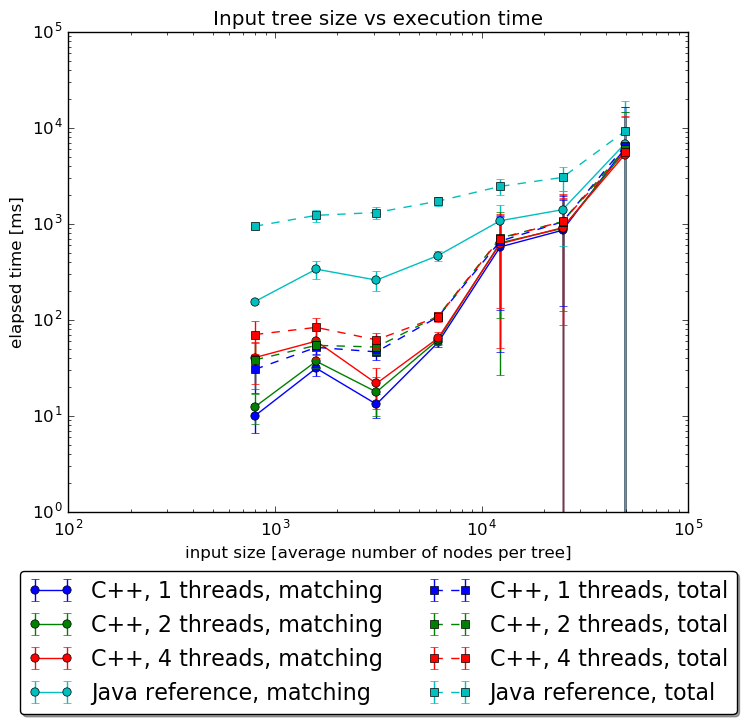
\includegraphics[width=\linewidth]{measurements/random/timePlot}
	\caption{Log-log plot of the execution time of the different implementations with various input sizes and 10 different randomly generated test cases for each input size. The bars show the standard deviation of the individual test cases from the mean execution time for that input size.}
	\label{fig:cpp_vs_java}
\end{figure}

\begin{figure}
	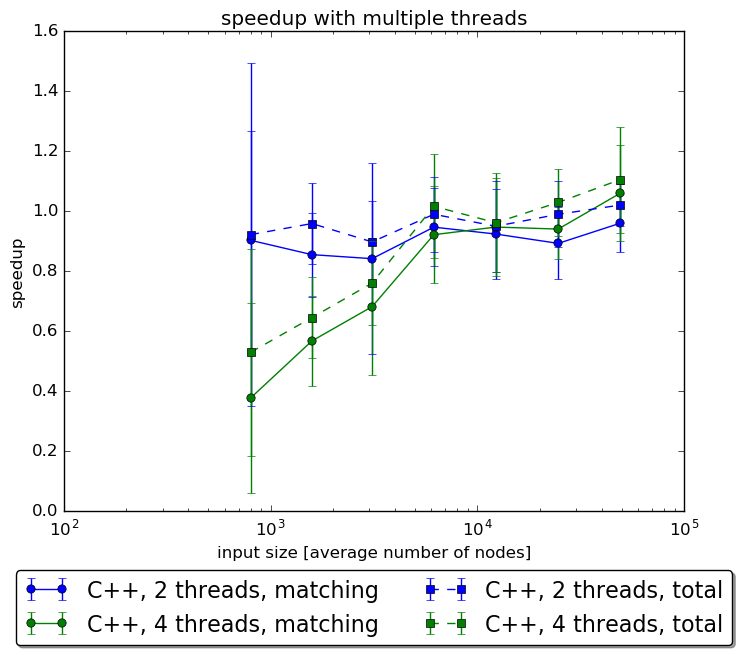
\includegraphics[width=\linewidth]{measurements/random/speedupPlot_c}
	\caption{Speedup compared to single threaded execution with various input sizes and 10 different randomly generated test cases for each input size. The bars show the standard deviation of the individual test cases from the mean speedup for that input size.}
	\label{fig:cpp_speedup}
\end{figure}

\mypar{Results on C++ ASTs}
The negative results with randomized test cases and the large differences between individual test cases of similar size prompted us to perform additional testing on real data.
Figure \ref{fig:electron_time} shows the execution time of the implementations on C++ ASTs with various input sizes.
The execution time of the reference implementation quickly grows to a point where further testing is unreasonable which is why data points for larger sizes are missing.
Presumably this is because of the missing search space reduction described in section \ref{sec:yourmethod} and it shows how essential that optimization is.
Regrettably we see similarly bad scaling behavior as with randomized tests with no significant speedup.

\begin{figure}
	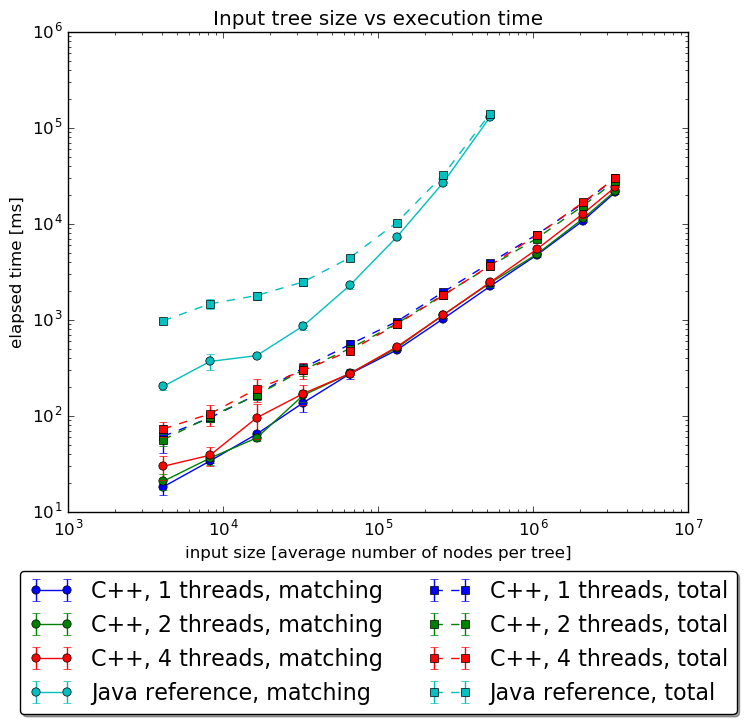
\includegraphics[width=\linewidth]{measurements/electron/timePlot}
	\caption{Log-log plot of the execution time of the different implementations with Electron ASTs truncated to different input sizes with 5 different test cases for each input size. The bars show the standard deviation of the individual test cases from the mean execution time for that input size.}
	\label{fig:electron_time}
\end{figure}

\section{Possible reasons for bad scaling}

In this section we explain what we believe are the reasons why our implementation scales badly and argue that achieving significant speedup through parallelization is unlikely.

While we could achieve substantially improved performance in comparison to the reference implementation, our implementation fails to benefit from multithreaded execution.
An important observation to make is that the proportion of the computation that is executed in parallel depends on the problem instance and is generally quite small.
The parallelized check for isomorphism is only executed for subtrees with matching hash values i.e. for identical subtrees or, with low probability, for different subtrees with identical hash values.
Furthermore we see that for a large majority of nodes, the candidate list in the bottom-up phase does not contain more than one candidate which makes it impossible to gain a speedup with multiple threads.

We believe that further improvements by parallelization would prove difficult because of the greedy nature of the \emph{Gumtree} algorithm.
Consider the main loop of the top-down phase (see Algorithm \ref{alg:top-down}, line 3).
The matchings computed in one iteration determine which subtrees will be considered in the next iteration.
This introduces a dependency between the iterations.
%In principle one could proceed with the iteration of a lower subtree height before the previous iteration has finished by iterating over but 

Parallelizing the loop over pairs of potentially isomorphic subtrees in the same phase (see line 12) is feasible and is likely beneficial to the algorithm in its original form.
With our optimization of reducing the search space however, the number of iterations and with it the potential benefit of parallelization is lowered drastically.
Especially so since the majority of iterations now result in a match being found and added to either $A$ or $M$, both data structures that need to be kept consistent which would introduce additional overhead.

The final loop of the top-down phase (see line 23) greedily decides on matchings to add to $M$ and, similar to the main loop, decisions made in earlier iterations determine which pairs are available in later iterations.

The main loop of the bottom-up phase (see Algorithm \ref{alg:bottom-up}, line 1) again has the same problems as the seeds and similarity values computed in one iteration may depend on matchings made in earlier iterations.

\section{Conclusions}

In a first step we have implemented the \emph{Gumtree} algorithm in C++.
We then found several sections in the algorithm that could be parallelized and used OpenMP to implement these parallelizations.
We also implemented an algorithmic optimization that turned out to be crucial.
To test and evaluate our implementation we needed many pairs of large similar trees so we implemented a randomized tree generator to create these test cases.
We also created test cases from the ASTs of the C++ project \emph{Electron}.

Our performance tests with randomly generated trees showed that while our implementation runs faster than the Java reference implementation, it does not scale with multiple threads.
Performance tests on real data confirmed the bad scaling behavior but showed that our implementation can in a few seconds solve instances which were previously unfeasible.
We think the reason for bad scaling is the fundamentally greedy nature of the \emph{Gumtree} algorithm.
This results in the proportion of the computational effort that is effectively parallelizable being quite small for typical ASTs.

% References should be produced using the bibtex program from suitable
% BiBTeX files (here: bibl_conf). The IEEEbib.bst bibliography
% style file from IEEE produces unsorted bibliography list.
% -------------------------------------------------------------------------
\bibliographystyle{IEEEbib}
\bibliography{bibl_conf}

\end{document}

